\epigraph{``Of course it is happening inside your head, Harry, but why on earth should that mean it is not real?"}{Albus Dumbledore}

\section{Performance Benchmark}
\subsection{Python vs. Cython Performance}
\begin{figure}[H]
    \centering
    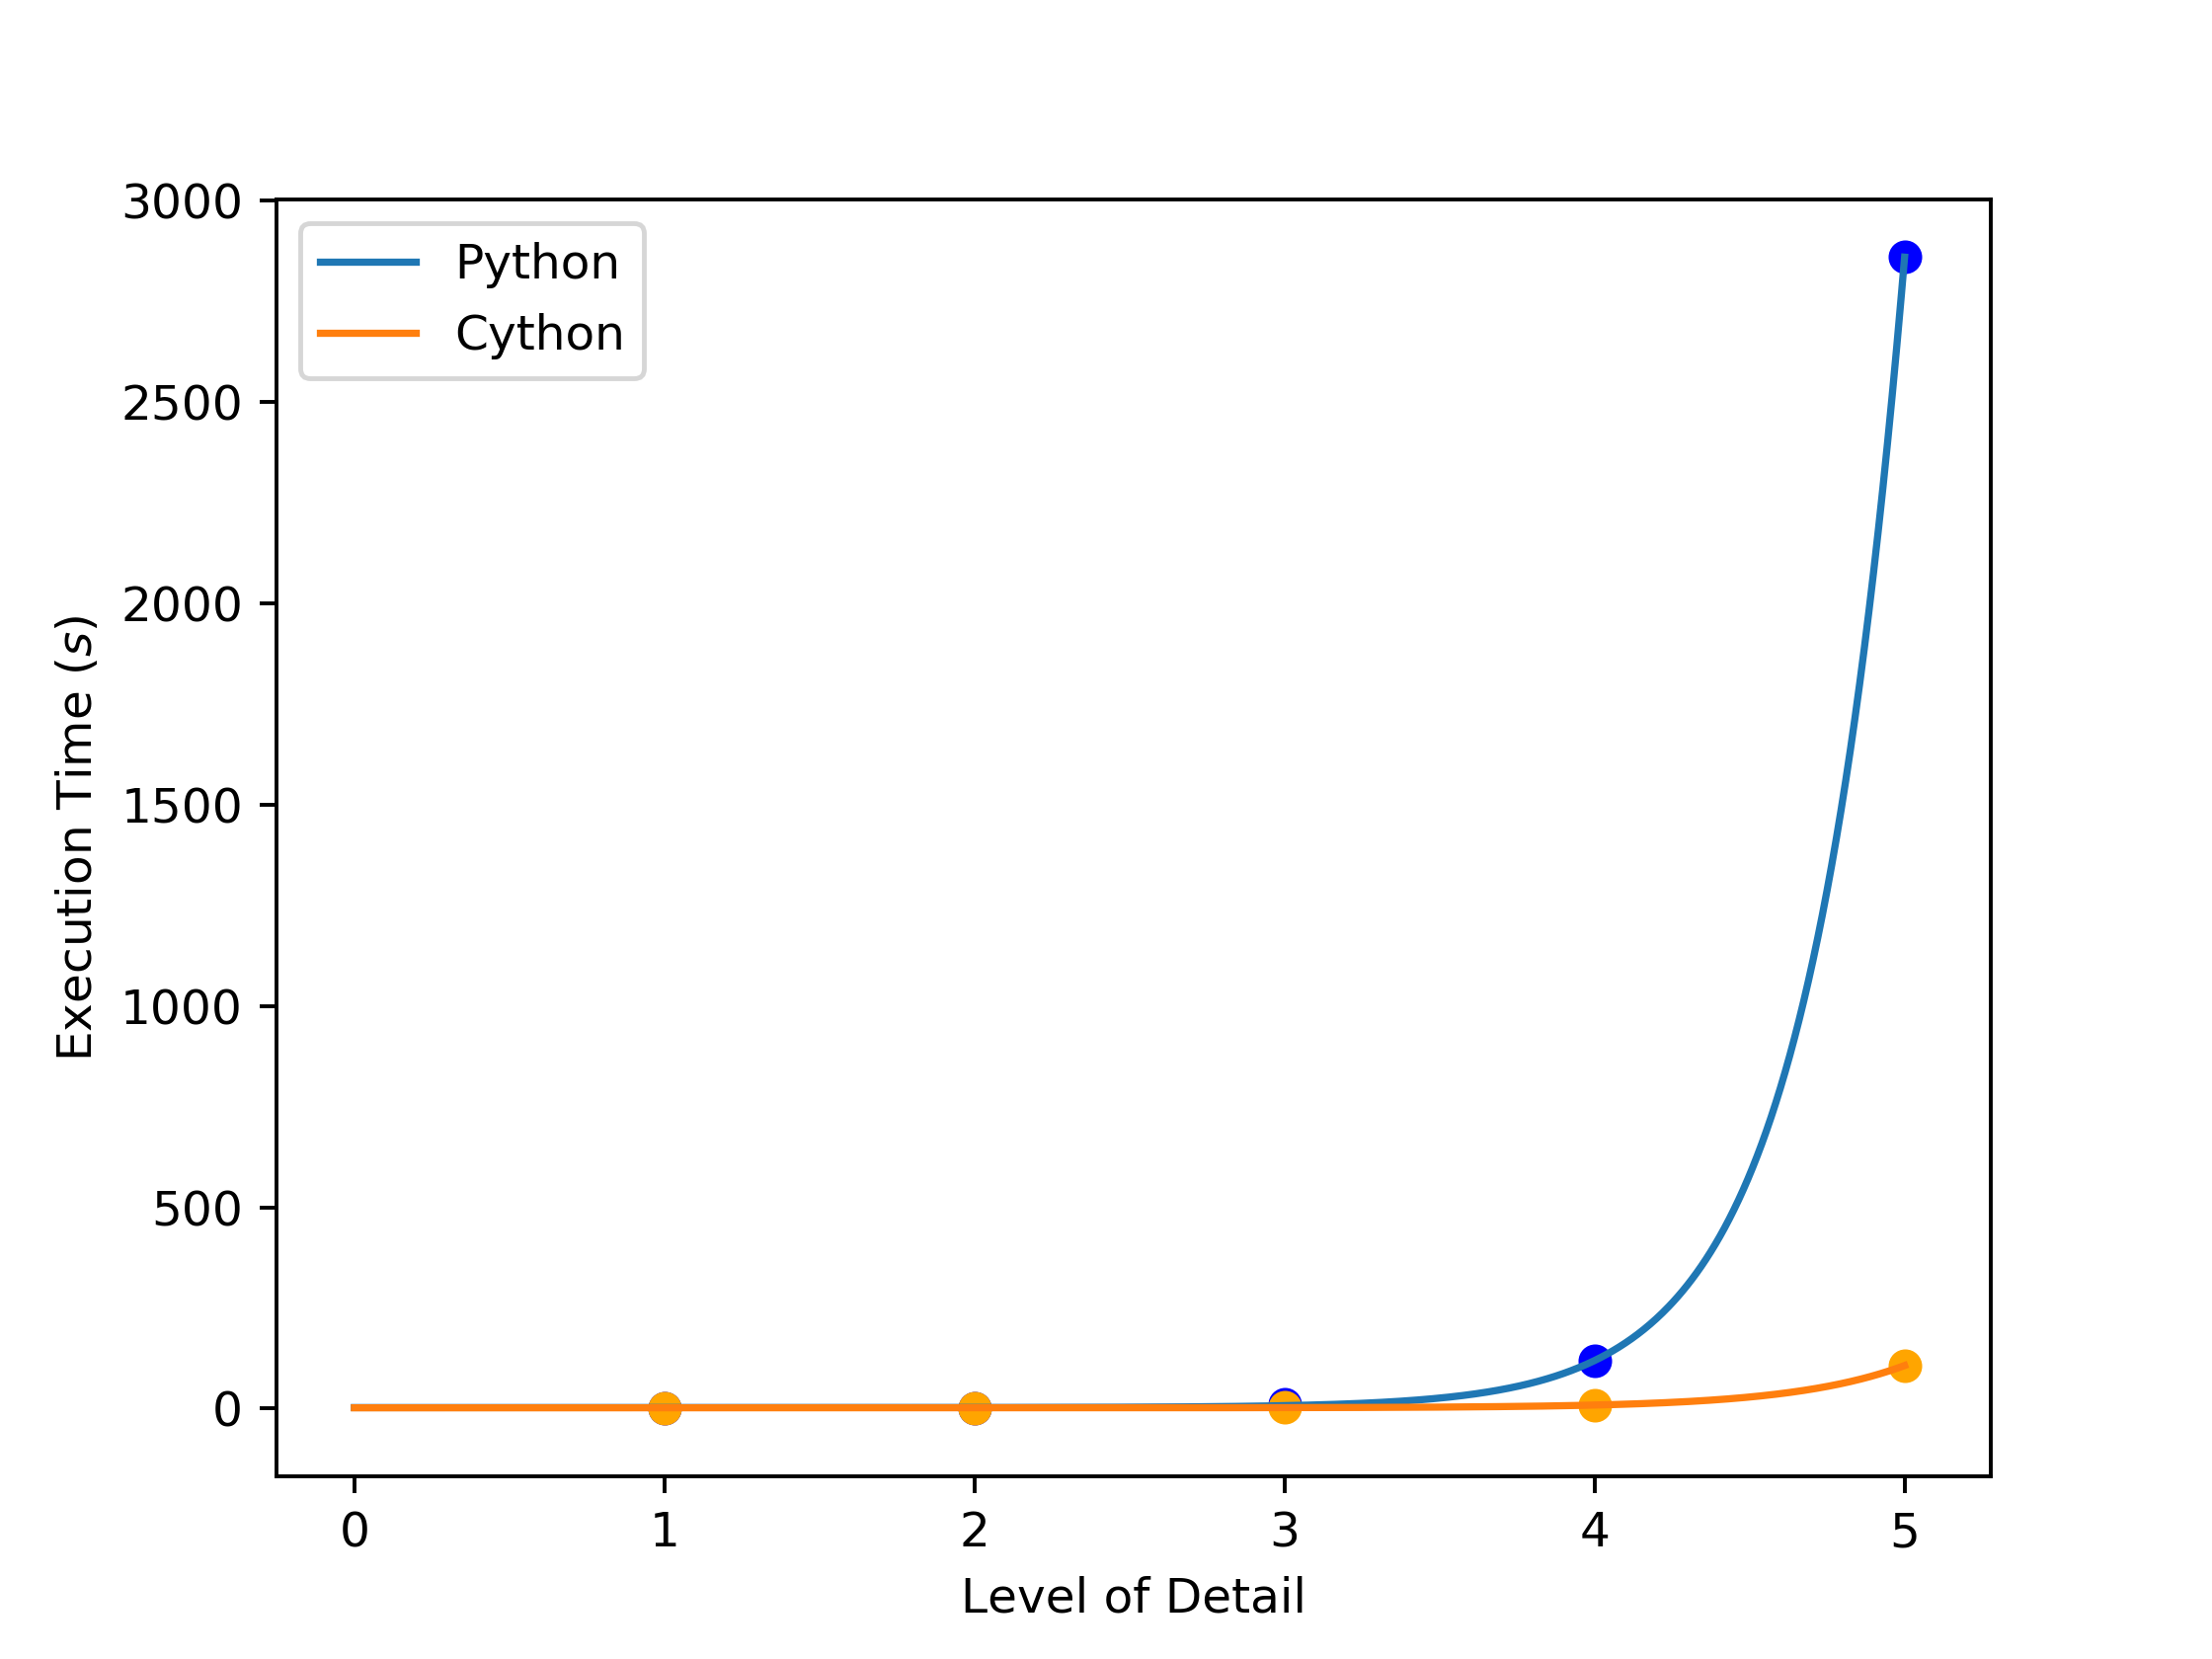
\includegraphics[width=.8\linewidth]{Graphs/python_vs_cython.png}
    \caption{AMSIMP Python vs. Cython Performance Benchmark}
    \label{python_vs_cython}
\end{figure}

The biggest difference in execution time, between the Cython version of AMSIMP and the Python version, can be observed at levels of detail 4 and 5, where the Cython version is on average over 25 times faster than the Python version of the software. When the software ultimately moves away from simulating atmospheric dynamics solely on a synoptic scale, this difference would only increase further.

\subsubsection{Statistical Analysis of the Results}
To demonstrate that using the programming language of Cython will result in a statistically significant increase in performance, it was decided to analyse the aforementioned results using Welch's t-test in order to determine the p-value of the null hypothesis. The primary reason for choosing Welch's t-test was than it did not assume an equal population variance. The null hypothesis states that `there is no significant difference in execution time between the Cython version of AMSIMP and the Python version'. The resulting p-value was 0.0009, hence thereof we can reject the null hypothesis. 

\subsection{Reliability of the Software's Performance}\label{stats}
\begin{center}
\begin{tabular}{|c|c|c|c|} 
 \hline
 Forecast Day & $\bar{x}$ & $\sigma$ & $\frac{\sigma}{\bar{x}}$ \\
 \hline
 1 & 48.71941 & 1.6192 & 0.03324 \\
 \hline
 2 & 82.05565 & 3.14003 & 0.03827 \\
 \hline
 3 & 122.0275 & 6.96494 & 0.05708 \\
 \hline
 4 & 164.84392 & 6.02163 & 0.03653 \\
 \hline
 5 & 209.37133 & 7.62972 & 0.03644 \\
 \hline
\end{tabular}\par
\bigskip
Table 6.1.: Reliability of the Software's Performance
\end{center}

To prove that the software is consistent and reliable, it was necessary to perform a statistical analysis. In order to do this, I examined the mean ($\bar{x}$), the standard deviation ($\sigma$), and the coefficient of variation ($\frac{\sigma}{\bar{x}}$) of the execution time of forecasts of various lengths. As a rule of thumb, a coefficient of variation $\geq$ 1 indicates a relatively high variation, while a coefficient of variation $<$ 1 can be considered low. The results of this statistical analysis are presented in the table above. This shows that all of the coefficient of variations values are well below 1, with the average coefficient of variation being 0.04.

\section{Accuracy Benchmark}
\begin{figure}[H]
    \centering
    \includegraphics[width=.8\linewidth]{Graphs/mape_graph.png}
    \caption{Prediction Accuracy of AMSIMP (MAPE)}
    \label{mape_accuracy}
\end{figure}

\begin{figure}[H]
    \centering
    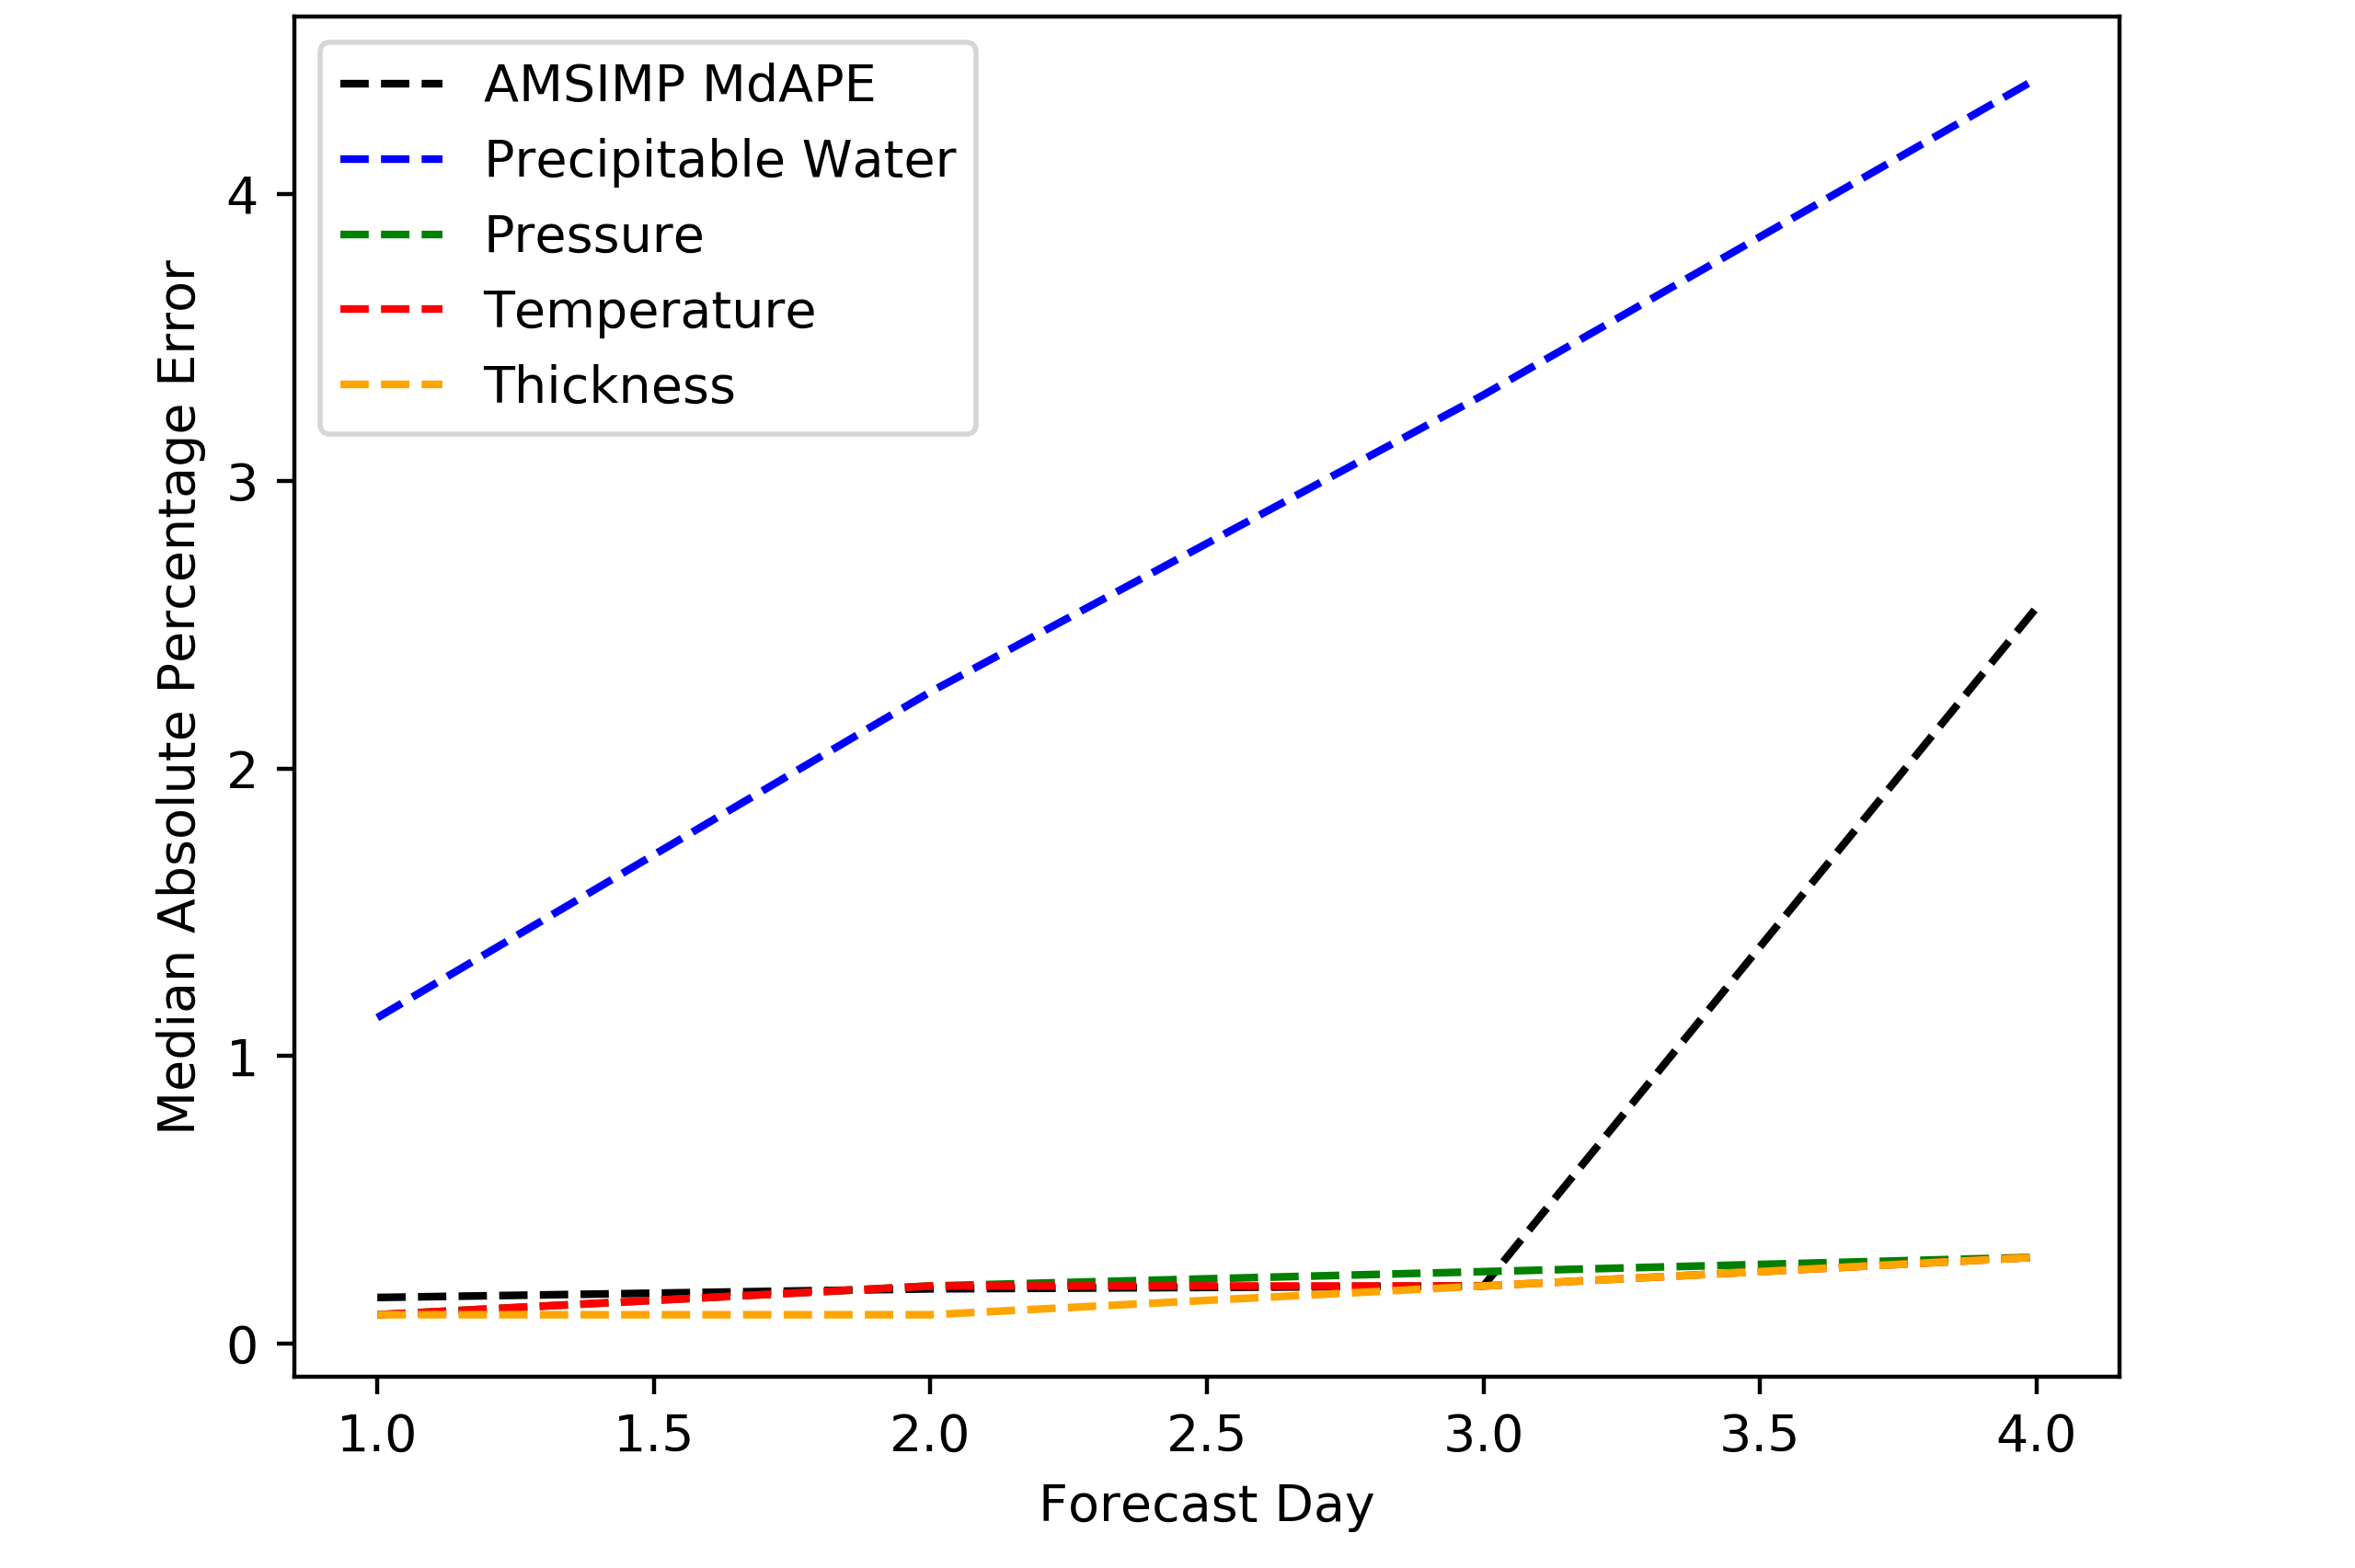
\includegraphics[width=.8\linewidth]{Graphs/mdape_graph.png}
    \caption{Prediction Accuracy of AMSIMP (MdAPE)}
    \label{mdape_accuracy}
\end{figure}

To further prove that the software is consistent and reliable, it was necessary to analyse the accuracy of the predictions produced by the software. The results of the benchmarking are presented in the graphs above. The software's mean absolute percentage error was approximately 1.56 \%, while the median absolute percentage error was approximately 0.81 \%. In order to determine whether the forecast produced was accurate or inaccurate based on the mean and median absolute percentage error, it was necessary to carry out a comparison in relation to something. To do this, I took the following table from the book entitled, `Industrial and business forecasting methods'\cite{mape}:

\hfill

\begin{center}
    \begin{tabular}{|c|c|} 
     \hline
     MAPE / MdAPE & Interpretation \\
     \hline
     $<10$  & Highly accurate forecasting \\
     \hline
     $\geq 10<20 $ & Good forecasting \\
     \hline
     $\geq 20<50 $ & Reasonable forecasting \\
     \hline
     $>50$ & Inaccurate forecasting \\
     \hline
    \end{tabular}\par
    \bigskip
    Table 6.2.: Interpretation of the Mean and Median Absolute Percentage Errors.
\end{center}

Considering that the highest mean absolute percentage error is below 7 \% and the highest median absolute percentage error is below 5 \%, one must interpret that the forecast produced by AMSIMP is highly accurate. It is, however, important to note at this stage that there is considerable debate as to whether there is a fixed cut off point for the mean and median absolute percentage errors. This is discussed at greater depth in chapter \ref{7}.

\section{Code Quality Benchmark}\label{PCQ}
In order to prove that the software consists of high quality source code, a series of benchmarking on the source code of the software was carried. The first benchmark consisted of utilising Pylint, a linter for Python, to generate an assessment on the source code. This assessment provided a numerical value, which could be compared against the table below to determine the code quality\cite{pylint}:

\hfill

\begin{center}
    \begin{tabular}{|c|c|} 
         \hline
         Numerical Rating & Interpretation \\
         \hline
         $<$ 0.0 & Trouble ahead \\
         \hline
         0.0 - 5.0 & Needs cleanup \\
         \hline
         5.0 - 7.0 & Reasonable quality \\
         \hline
         $>$ 7.0 & Great code! \\
         \hline
    \end{tabular}\par  
    \bigskip
    Table 6.3.: Interpretation of the numerical rating provided by Pylint.
\end{center}

The second benchmark consisted of utilising Coverage.py, and Codecov to generate a report on the overall code coverage of the software. A high code coverage, above approximately 80 \%, tells us that a piece of software has more of its source code executed during testing, which implies that the software has a lower chance of containing undetected bugs, ultimately demonstrating that the quality of the source code is high.

\subsection{Linting Benchmark}
\begin{figure}[H]
    \centering
    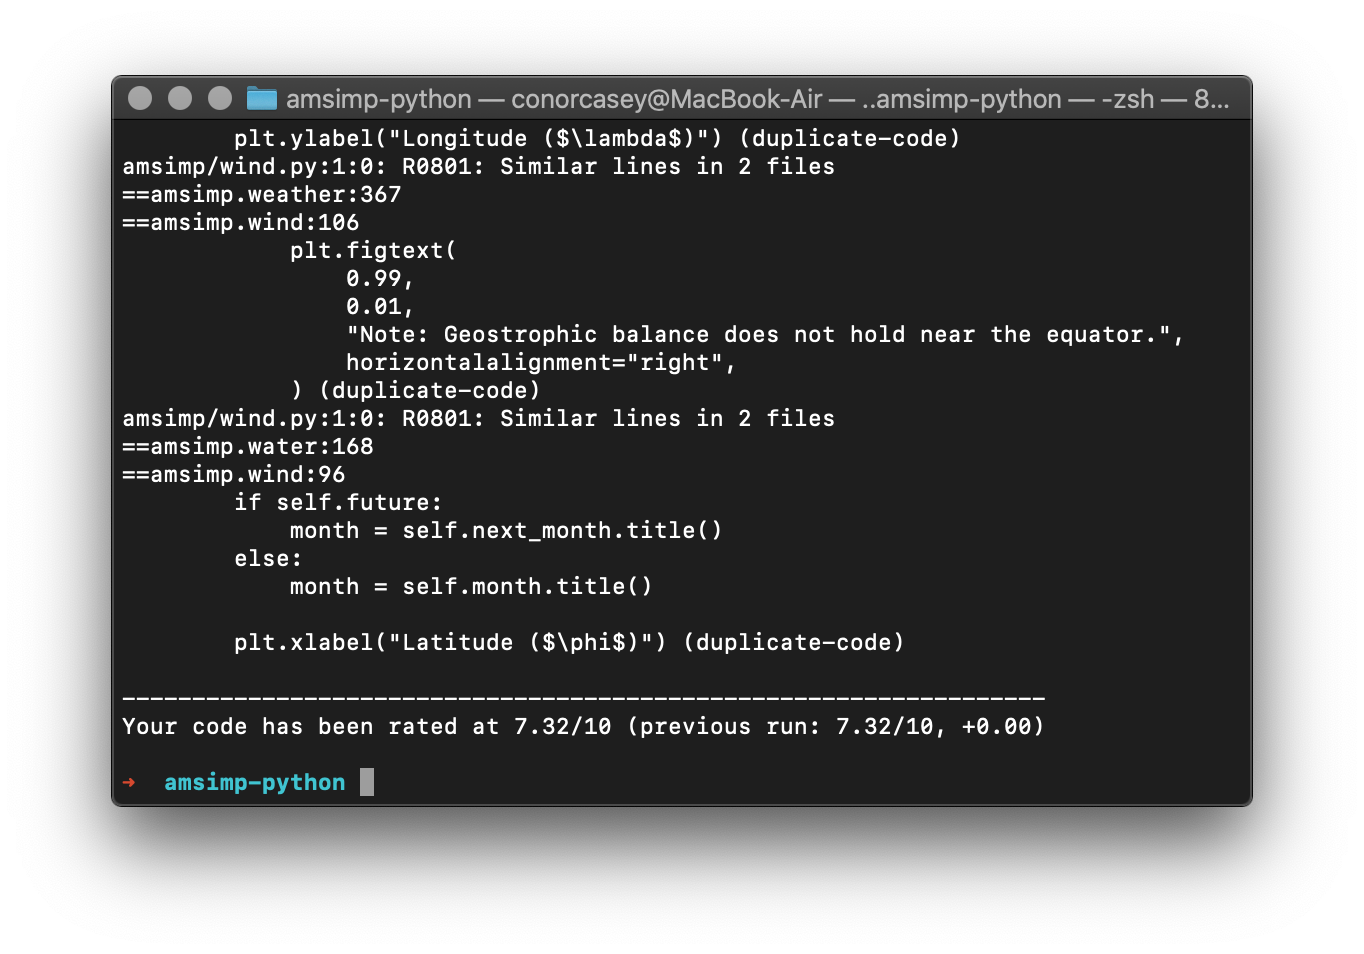
\includegraphics[width=.7\linewidth]{Images/code_quality}
    \caption{The Python linter, Pylint, assessment of the quality of the source code of the software.}
    \label{code_quality}
\end{figure}

The assessment of the source code of the software by Pylint is presented above. The numerical rating, as provided, is approximately 7.32. Please note that this benchmark was performed on AMSIMP v0.1.6.

\subsection{Coverage Benchmark}
\begin{figure}[H]
    \centering
    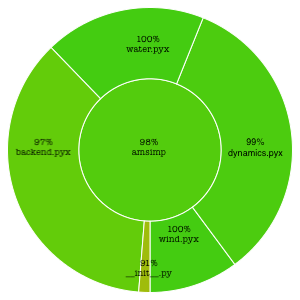
\includegraphics[width=.4\linewidth]{Images/code_coverage.png}
    \caption{The code coverage of the software.}
    \label{code_coverage}
\end{figure}

The results of the code coverage test are presented in the graph above, with the mean code coverage for the software being approximately 98 \%. Please note that this benchmark was performed on AMSIMP v0.3.4. 
